\documentclass[a4paper,14pt]{article} 


\usepackage{fontenc}			
\usepackage[utf8]{inputenc}			
\usepackage[english,russian]{babel}	

\usepackage{graphicx, scalerel}    
\usepackage{wrapfig}               
\usepackage[14pt]{extsizes}        
\usepackage[warn]{mathtext}       
\usepackage{indentfirst}      
\usepackage{geometry}
\usepackage[table,xcdraw]{xcolor} 
\usepackage{amsmath,amsfonts,amssymb,amsthm,mathtools}
\usepackage{wasysym}                
\usepackage{upgreek}                
\usepackage{caption}
\usepackage{multirow}
\captionsetup{labelsep=period}
\usepackage[font=small,labelfont=bf]{caption}
\usepackage{gensymb}
\usepackage[unicode, pdftex]{hyperref}
\usepackage{fancyhdr}
\setlength\fboxsep{3pt}
\setlength\fboxrule{1pt}
\usepackage{tocloft}
\usepackage[pdftex]{lscape}
\usepackage{icomma}
\setlength{\arrayrulewidth}{0.4mm}
\usepackage{setspace}
\usepackage{pdfpages}
\usepackage{cmap}

\graphicspath{pictures/}


\newcommand{\tocsection}[1]{\section*{#1} \addcontentsline{toc}{section}{#1}}
\newcommand{\tocsubsection}[1]{\subsection*{#1} \addcontentsline{toc}{subsection}{#1}}
\renewcommand{\cftsecleader}{\cftdotfill{\cftdotsep}}

\newcommand{\comment}[1]{}


\geometry{a4paper,
		  total={170mm,257mm},
		  left=30mm,
		  right=15mm,
		  top=20mm,
		  bottom=20mm}
\onehalfspacing
\setlength{\parindent}{12.5mm}

\bibliographystyle{plain}


\begin{document}
	\newcommand{\HRule}{\rule{\linewidth}{0.7mm}}

\begin{center}
	\large\textbf{Московский Физико-Технический Институт}\\
	\vfill
		
	\Large Микроархитектура современных микропроцессоров
	\\[0.4cm]
	{ \huge \bfseries Replacement Policies}
	\\[0.4cm]
	
	\ \\
	\textbf{\large Автор:} \\	
	\large Овсянников Михаил\\
	\vfill
	\large Долгопрудный, 2025
\end{center}

\thispagestyle{empty}

\newpage
\setcounter{page}{2}

	
	\section*{Политики замещения}

	В качестве второго задания необходимо было исследовать различные политики замещения для кэшей (replacement policies). Для бенчмаркинга использовался симулятор \href{https://github.com/ChampSim/ChampSim}{ChampSim} и некоторый набор трасс SPEC CPU 2017 из DPC-3, предназначенный специально для него.
	
	Для оценки производительности политик замещения использовался процент промахов в кэш (Miss Rate), усредненный по всем используемым трассам с помощью геометрического среднего. Рассматриваемый кэш -- L2 кэш (кэш второго уровня).
	
	В качестве базовых политик замещения использовались LRU и DRRIP. Самостоятельно были реализованы политики Pseudo-LRU, MRU и LFU. Было проведено сравнение всех пяти политик. Ожидания по результатам следующие:
	\begin{itemize}
		\item DRRIP лучше, чем LRU
		\item LRU совсем немного лучше, чем Pseudo-LRU
		\item MRU в целом покажет достаточно плохие результаты
		\item LFU выдаёт результаты на уровне LRU
	\end{itemize}
	
	Ниже представлены результаты замеров Miss Rate в L2 кэш для разных политик замещения.
	
	\begin{figure}[h!]
		\centering
		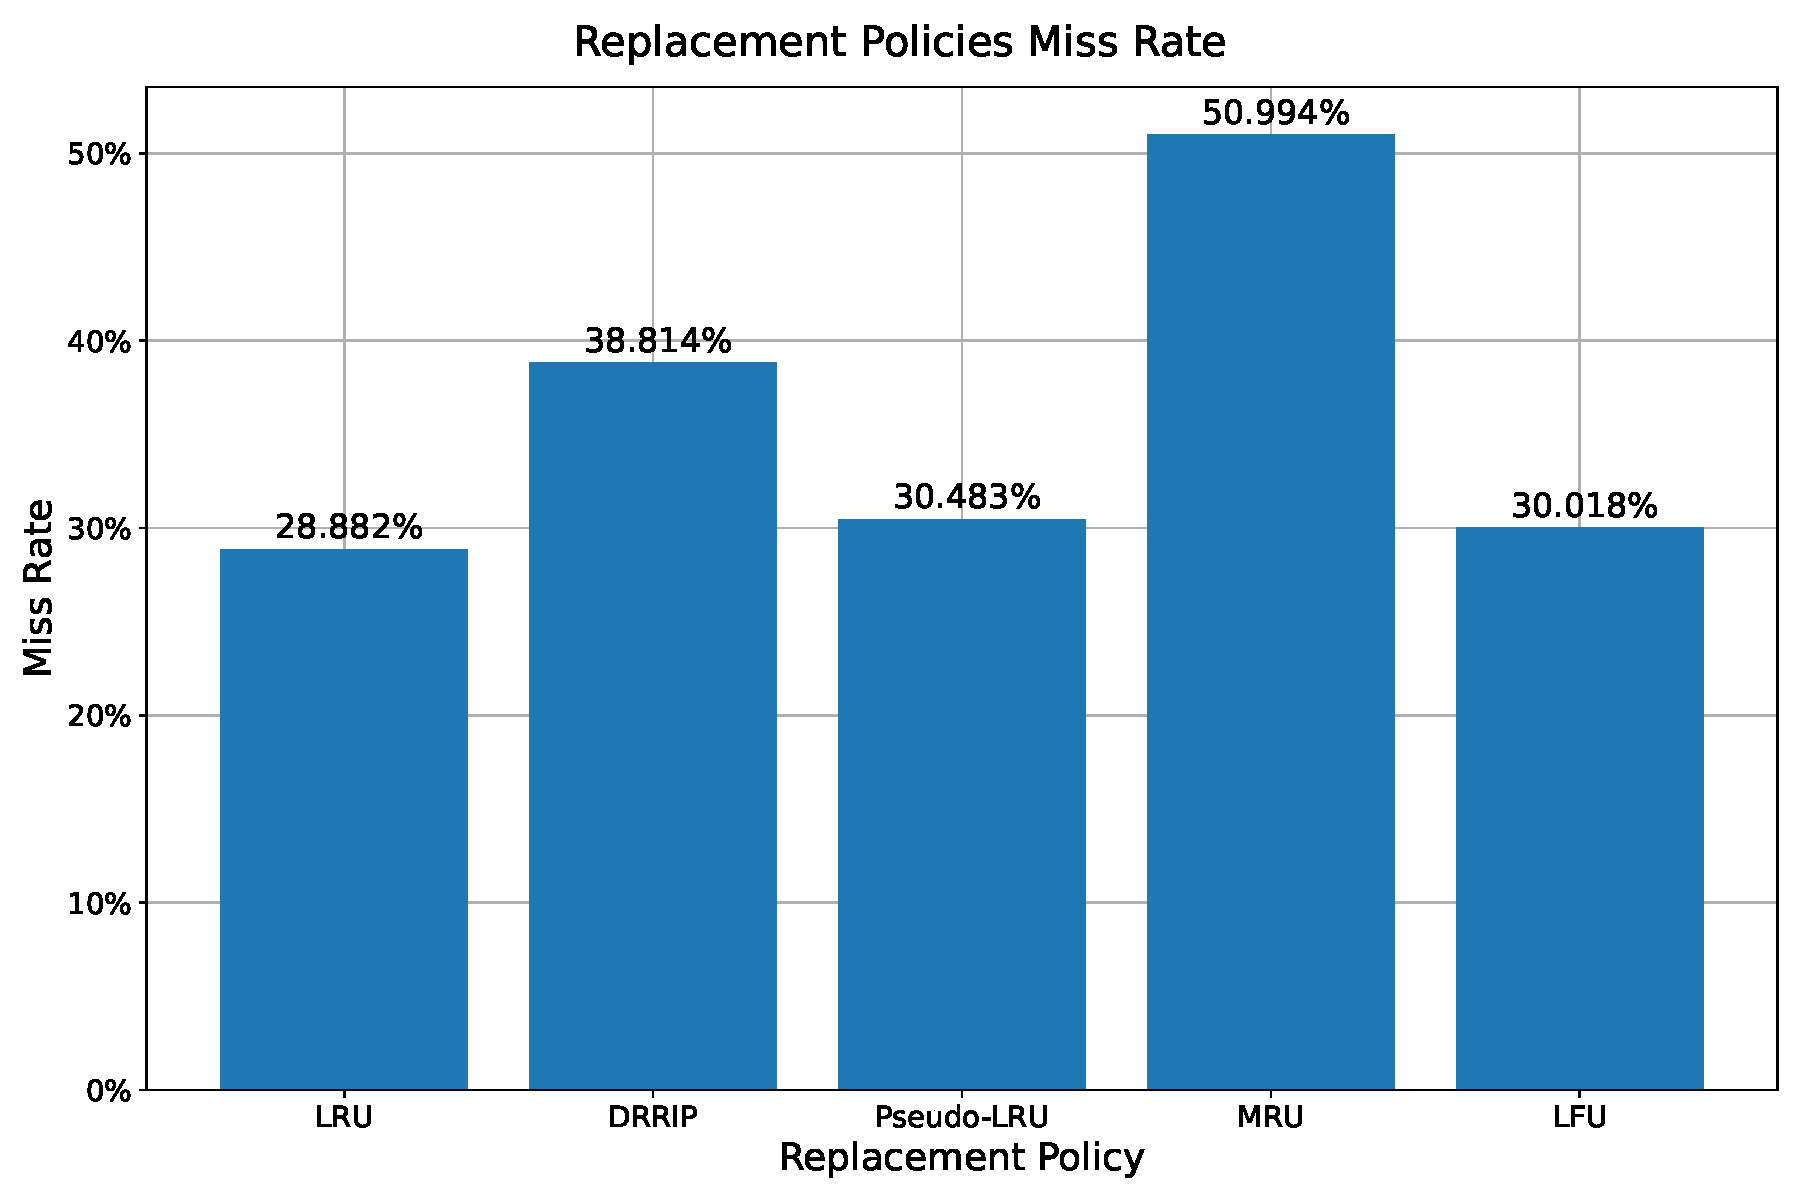
\includegraphics[width=\linewidth]{./pictures/miss_rate_gmean.pdf}
		\caption{Miss Rate в L2 кэш разных политик замещения}
	\end{figure}
	
	\newpage
	Заметим, что ожидания по результатам лишь частично оправдались.
	
	DRRIP оказался сильно хуже, чем LRU -- полная противоположность ожидаемому результату. Поскольку ни одна из этих политик замещения не было реализована самостоятельно, то это можно объяснить лишь несостоятельной реализацией DRRIP в симуляторе \href{https://github.com/ChampSim/ChampSim}{ChampSim}.
	
	Предсказание о том, что LRU лишь немного лучше Pseudo-LRU, сбылось. Разница лишь $\thicksim 5 \%$. Объяснение -- Pseudo-LRU является лишь приближением истинного LRU. В LRU вытесняется всегда самая старая ячейка, а в Pseudo-LRU -- не самая поздняя. В этом и состоит приближение. Если часто происходит обращение к нескольким ячейкам, то в LRU они не будут вытеснены, а в Pseudo-LRU такой гарантии нет.
	
	Также можно заметить, что политика MRU действительно оказалась достаточно плохой. Более половины обращений в кэш -- это промах! Очевидное объяснение этого -- MRU вытесняет самые поздние ячейки, что полностью противоречит необходимому действию в присутствии временной локальности (которая почти всегда имеет место быть).
	
	Ожидания по поводу LFU также оправдались -- данная политика действительно показала себя на уровне обычного LRU, уступая ей всего лишь на $\thicksim 4 \%$.
	
	\newpage
	
	\section*{Вывод}
	В этом задании были исследованы различные политики замещения кэшей. Проведено сравнение следующих: LRU, DRRIP, Pseudo-LRU, MRU и LFU. По результатам бенчмаркинга оказалось следующее:
	\begin{itemize}
		\item DRRIP сильно уступает стандартному LRU
		\item Pseudo-LRU немного хуже LRU и является хорошим его приближением
		\item MRU показал ожидаемо плохие результаты
		\item LFU показал ожидаемо хорошие результаты
	\end{itemize}

	\newpage
	\section*{Приложение}
	Ниже представлен график Miss Rate в L2 кэш для каждой трассы для более детального рассмотрения результатов. Номер по оси абсцисс -- это номер трассы.

	\newpage
	\newgeometry{left=0.1cm,right=0.1cm,top=0cm,bottom=0cm}
	\thispagestyle{empty}
	\begin{landscape}
		\vspace*{\fill}
		\begin{figure}[h!]
			\centering
			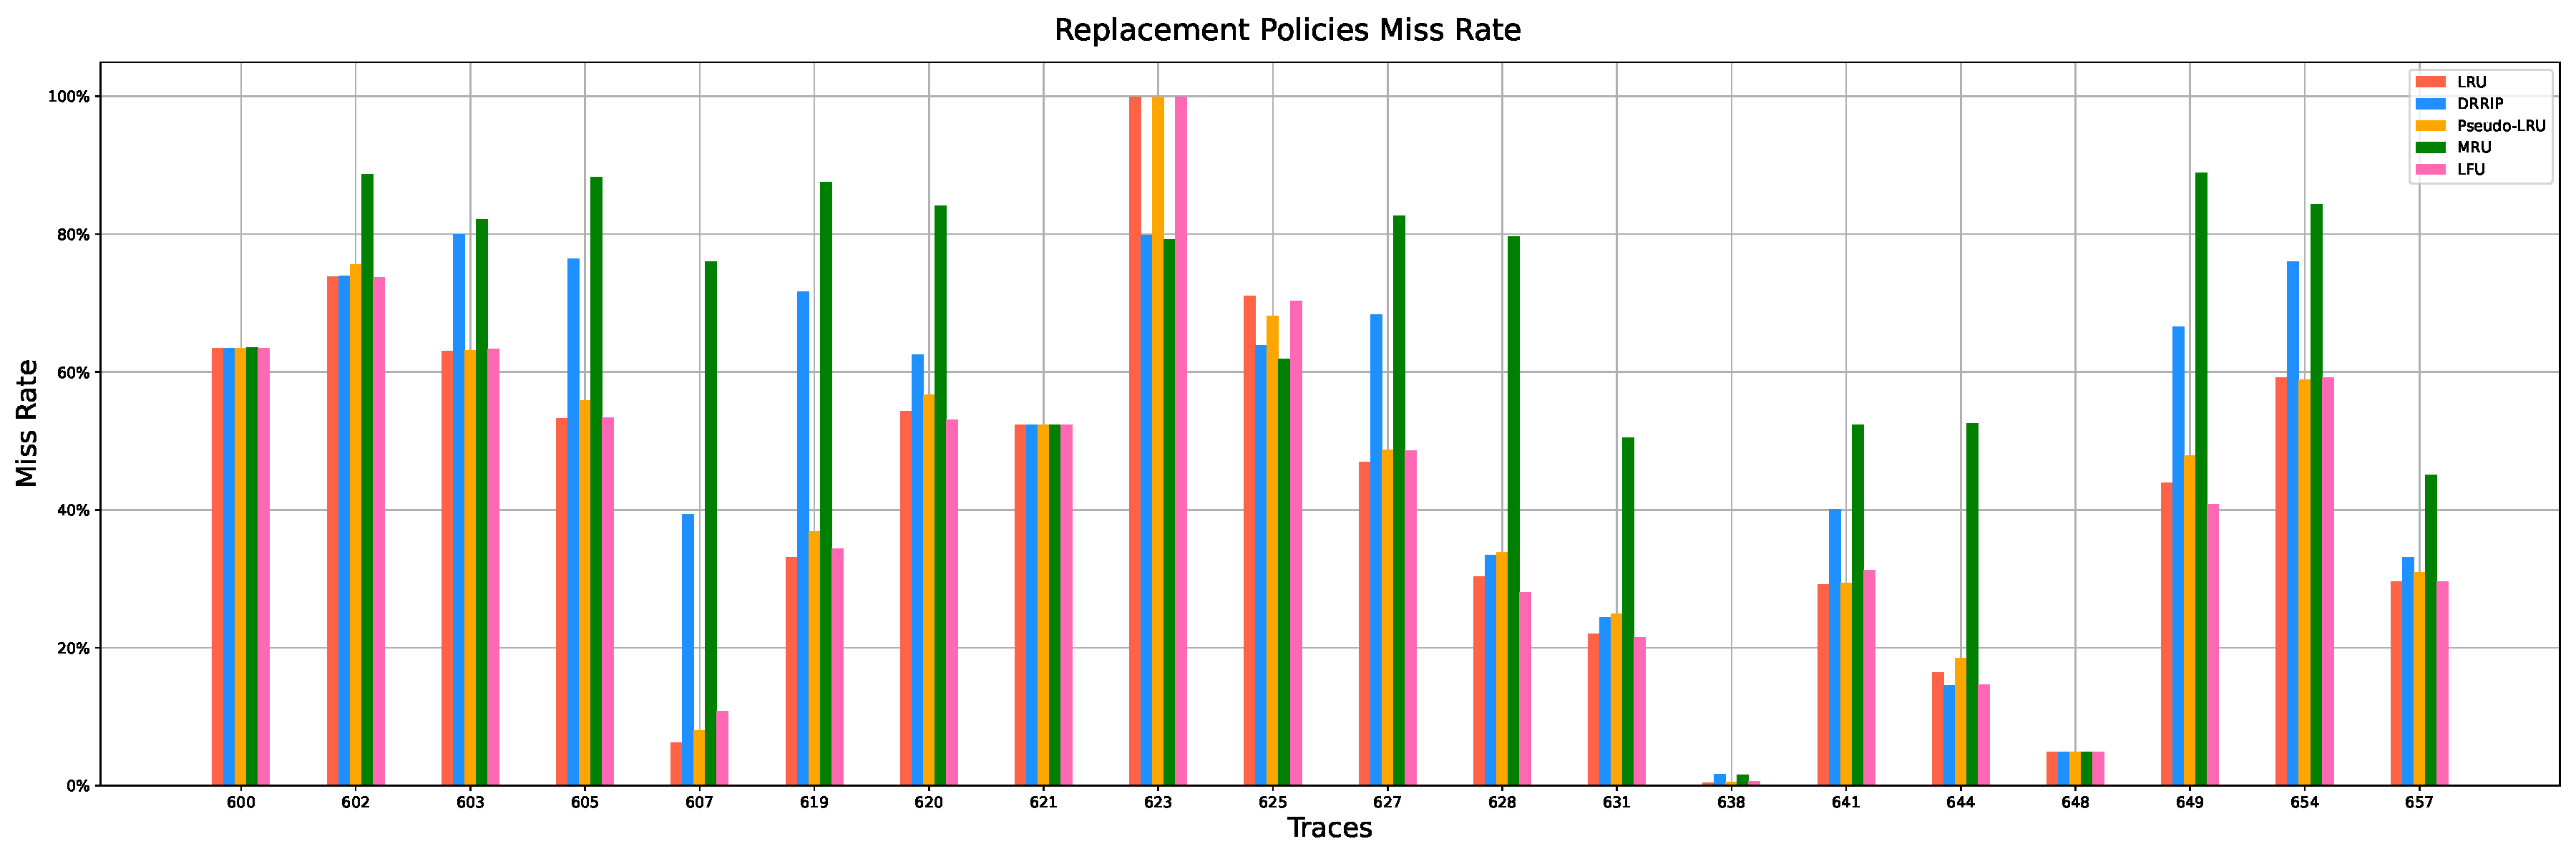
\includegraphics[width=\linewidth]{./pictures/miss_rate_traces.pdf}
		\end{figure}
		\vspace*{\fill}
	\end{landscape}

\end{document}